\documentclass{standalone}
\usepackage{tikz}
\usetikzlibrary{patterns, positioning}
\usepackage[sfdefault]{ClearSans} %% option 'sfdefault' activates Clear Sans as the default text font
\usepackage[T1]{fontenc}

\begin{document}
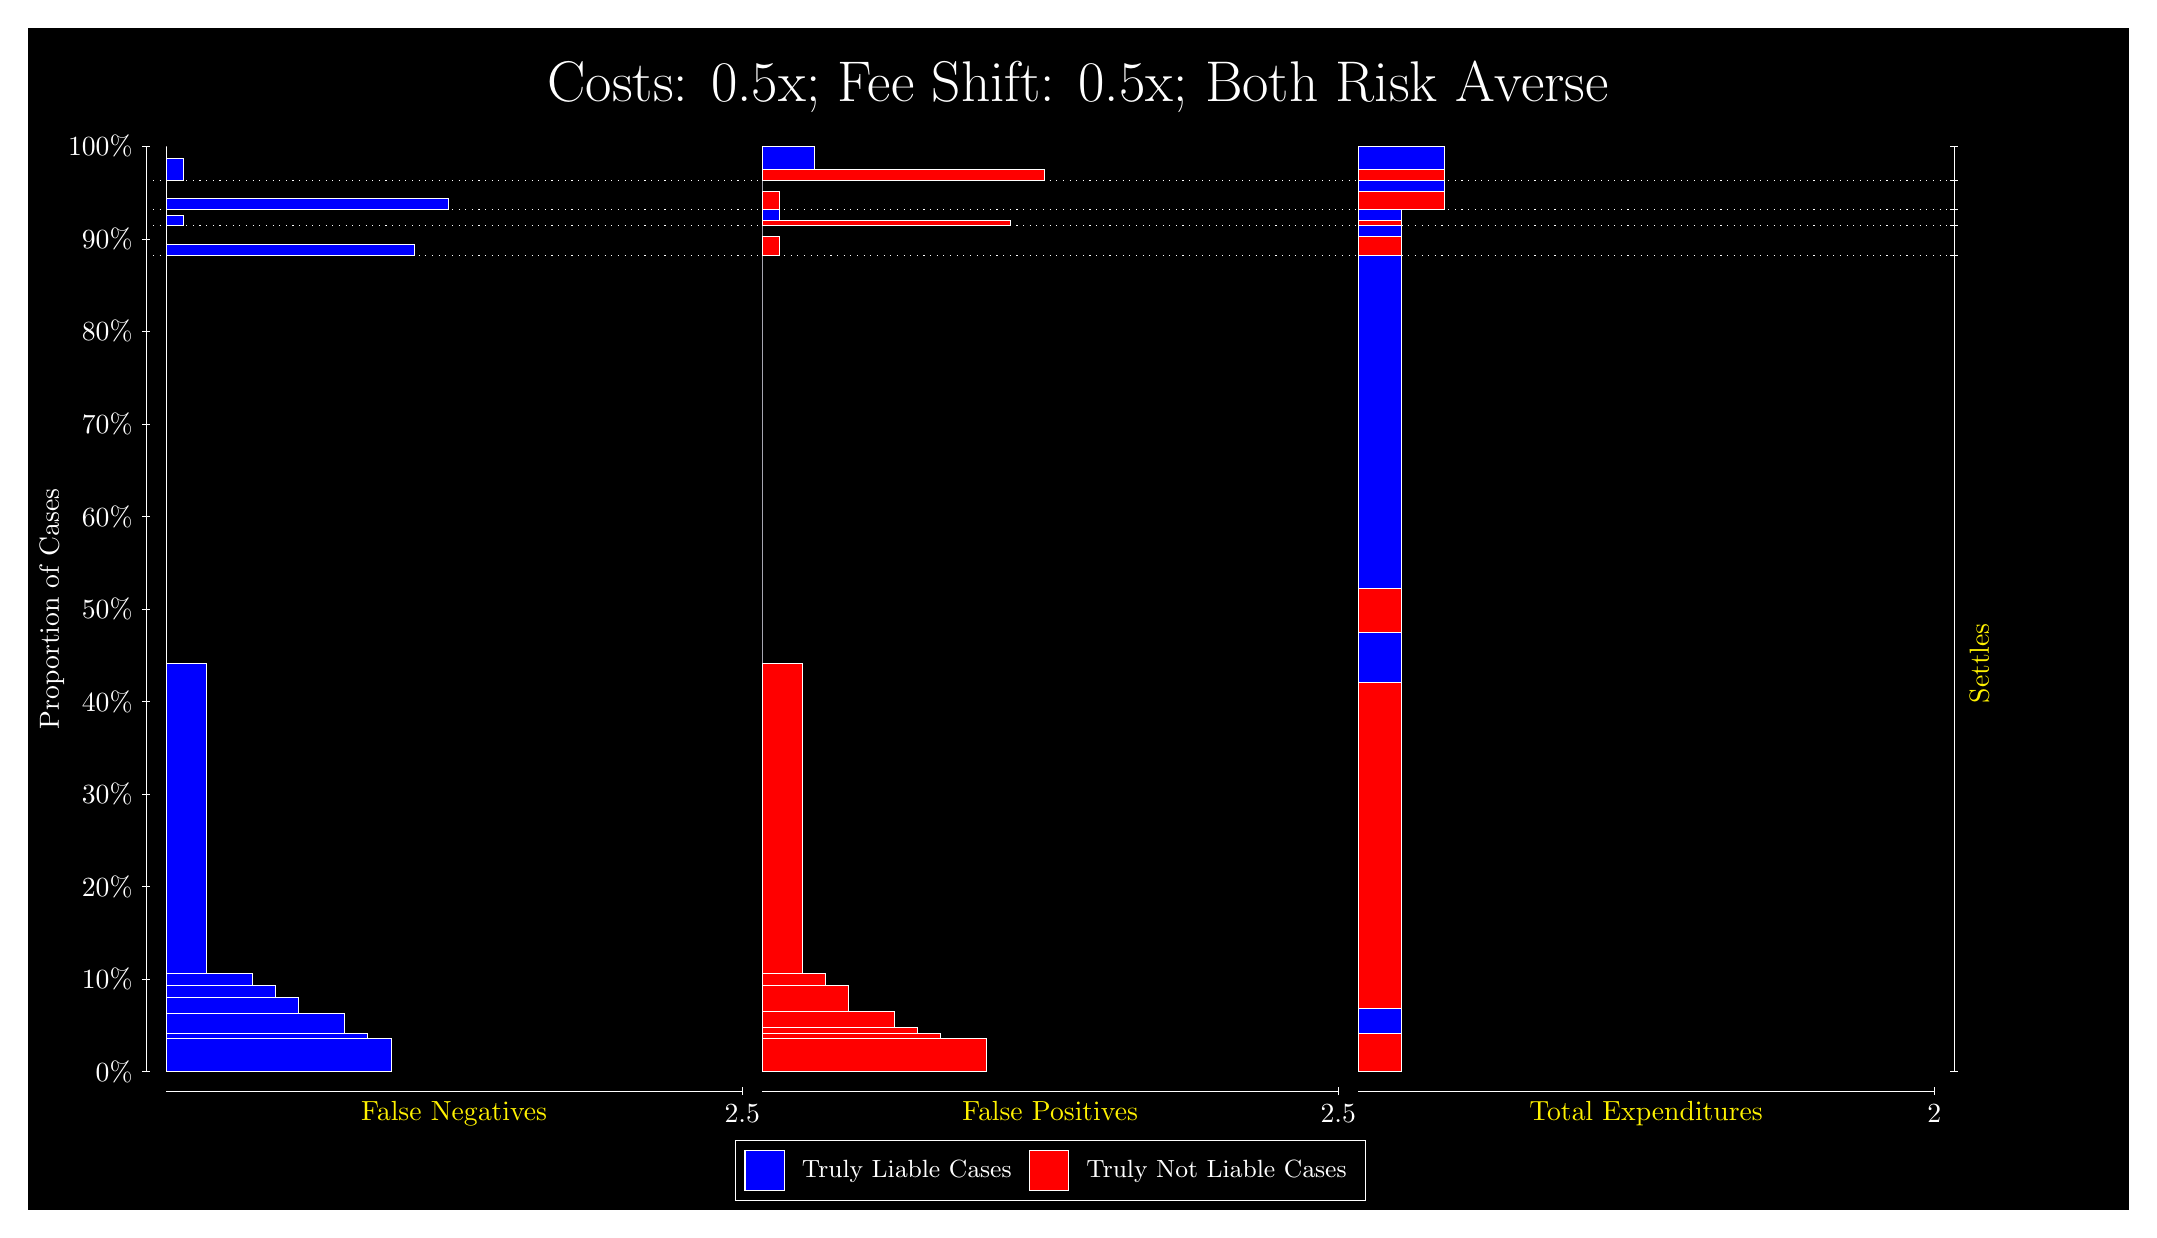
\begin{tikzpicture}
\draw[fill=black] (0,0) rectangle (26.667,15);
\draw[text=white] (0,13.5) rectangle (26.667,15) node[midway] {\huge Costs: 0.5x; Fee Shift: 0.5x; Both Risk Averse};
\draw[white, very thin] (1.5,1.75) -- (1.5,13.5);
\node[rotate=90, text=white, anchor=center] at (0.3, 7.625) {Proportion of Cases};
\draw[white, very thin] (1.45,1.75) -- (1.55,1.75);
\node[text=white, anchor=east] at (1.45, 1.75) {0\%};
\draw[white, very thin] (1.45,2.925) -- (1.55,2.925);
\node[text=white, anchor=east] at (1.45, 2.925) {10\%};
\draw[white, very thin] (1.45,4.1) -- (1.55,4.1);
\node[text=white, anchor=east] at (1.45, 4.1) {20\%};
\draw[white, very thin] (1.45,5.275) -- (1.55,5.275);
\node[text=white, anchor=east] at (1.45, 5.275) {30\%};
\draw[white, very thin] (1.45,6.45) -- (1.55,6.45);
\node[text=white, anchor=east] at (1.45, 6.45) {40\%};
\draw[white, very thin] (1.45,7.625) -- (1.55,7.625);
\node[text=white, anchor=east] at (1.45, 7.625) {50\%};
\draw[white, very thin] (1.45,8.8) -- (1.55,8.8);
\node[text=white, anchor=east] at (1.45, 8.8) {60\%};
\draw[white, very thin] (1.45,9.975) -- (1.55,9.975);
\node[text=white, anchor=east] at (1.45, 9.975) {70\%};
\draw[white, very thin] (1.45,11.15) -- (1.55,11.15);
\node[text=white, anchor=east] at (1.45, 11.15) {80\%};
\draw[white, very thin] (1.45,12.325) -- (1.55,12.325);
\node[text=white, anchor=east] at (1.45, 12.325) {90\%};
\draw[white, very thin] (1.45,13.5) -- (1.55,13.5);
\node[text=white, anchor=east] at (1.45, 13.5) {100\%};

\draw[white, very thin] (24.457,1.75) -- (24.457,13.5);
\draw[white, very thin] (24.407,1.75) -- (24.507,1.75);
\node[anchor=west] at (24.407, 1.75) {};
\draw[white, very thin] (24.407,12.119) -- (24.507,12.119);
\node[anchor=west] at (24.407, 12.119) {};
\draw[white, very thin] (24.407,12.495) -- (24.507,12.495);
\node[anchor=west] at (24.407, 12.495) {};
\draw[white, very thin] (24.407,12.701) -- (24.507,12.701);
\node[anchor=west] at (24.407, 12.701) {};
\draw[white, very thin] (24.407,13.064) -- (24.507,13.064);
\node[anchor=west] at (24.407, 13.064) {};
\draw[white, very thin] (24.407,13.5) -- (24.507,13.5);
\node[anchor=west] at (24.407, 13.5) {};

\draw[white, very thin, fill=blue] (1.75,1.75) rectangle (4.6044,2.1734);
\draw[white, very thin, fill=blue] (1.75,2.1734) rectangle (4.3116,2.2396);
\draw[white, very thin, fill=blue] (1.75,2.2396) rectangle (4.0188,2.4881);
\draw[white, very thin, fill=blue] (1.75,2.4881) rectangle (3.4333,2.6976);
\draw[white, very thin, fill=blue] (1.75,2.6976) rectangle (3.1406,2.8478);
\draw[white, very thin, fill=blue] (1.75,2.8478) rectangle (2.8478,2.998);
\draw[white, very thin, fill=blue] (1.75,2.998) rectangle (2.2623,6.9347);
\draw[white, very thin, fill=red] (1.75,6.9347) rectangle (1.75,12.119);
\draw[white, very thin, fill=blue] (1.75,12.119) rectangle (4.8971,12.252);
\draw[white, very thin, fill=red] (1.75,12.252) rectangle (1.75,12.495);
\draw[white, very thin, fill=blue] (1.75,12.495) rectangle (1.9696,12.628);
\draw[white, very thin, fill=red] (1.75,12.628) rectangle (1.75,12.701);
\draw[white, very thin, fill=blue] (1.75,12.701) rectangle (5.3362,12.837);
\draw[white, very thin, fill=red] (1.75,12.837) rectangle (1.75,13.064);
\draw[white, very thin, fill=blue] (1.75,13.064) rectangle (1.9696,13.353);
\draw[white, very thin, fill=red] (1.75,13.353) rectangle (1.75,13.5);
\draw[white, very thin, fill=red] (9.3189,1.75) rectangle (12.173,2.1734);
\draw[white, very thin, fill=red] (9.3189,2.1734) rectangle (11.588,2.2396);
\draw[white, very thin, fill=red] (9.3189,2.2396) rectangle (11.295,2.3058);
\draw[white, very thin, fill=red] (9.3189,2.3058) rectangle (11.002,2.5154);
\draw[white, very thin, fill=red] (9.3189,2.5154) rectangle (10.417,2.8478);
\draw[white, very thin, fill=red] (9.3189,2.8478) rectangle (10.124,2.998);
\draw[white, very thin, fill=red] (9.3189,2.998) rectangle (9.8312,6.9347);
\draw[white, very thin, fill=blue] (9.3189,6.9347) rectangle (9.3189,12.119);
\draw[white, very thin, fill=red] (9.3189,12.119) rectangle (9.5384,12.362);
\draw[white, very thin, fill=blue] (9.3189,12.362) rectangle (9.3189,12.495);
\draw[white, very thin, fill=red] (9.3189,12.495) rectangle (12.466,12.567);
\draw[white, very thin, fill=blue] (9.3189,12.567) rectangle (9.5384,12.701);
\draw[white, very thin, fill=red] (9.3189,12.701) rectangle (9.5384,12.928);
\draw[white, very thin, fill=blue] (9.3189,12.928) rectangle (9.3189,13.064);
\draw[white, very thin, fill=red] (9.3189,13.064) rectangle (12.905,13.212);
\draw[white, very thin, fill=blue] (9.3189,13.212) rectangle (9.9776,13.5);
\draw[white, very thin, fill=red] (16.888,1.75) rectangle (17.437,2.2326);
\draw[white, very thin, fill=blue] (16.888,2.2326) rectangle (17.437,2.5473);
\draw[white, very thin, fill=red] (16.888,2.5473) rectangle (17.437,6.6935);
\draw[white, very thin, fill=blue] (16.888,6.6935) rectangle (17.437,7.3264);
\draw[white, very thin, fill=red] (16.888,7.3264) rectangle (17.437,7.8823);
\draw[white, very thin, fill=blue] (16.888,7.8823) rectangle (17.437,12.119);
\draw[white, very thin, fill=red] (16.888,12.119) rectangle (17.437,12.362);
\draw[white, very thin, fill=blue] (16.888,12.362) rectangle (17.437,12.495);
\draw[white, very thin, fill=red] (16.888,12.495) rectangle (17.437,12.567);
\draw[white, very thin, fill=blue] (16.888,12.567) rectangle (17.437,12.701);
\draw[white, very thin, fill=red] (16.888,12.701) rectangle (17.986,12.928);
\draw[white, very thin, fill=blue] (16.888,12.928) rectangle (17.986,13.064);
\draw[white, very thin, fill=red] (16.888,13.064) rectangle (17.986,13.212);
\draw[white, very thin, fill=blue] (16.888,13.212) rectangle (17.986,13.5);
\draw[white, dotted] (1.5,12.119) -- (24.457,12.119);
\draw[white, dotted] (1.5,12.495) -- (24.457,12.495);
\draw[white, dotted] (1.5,12.701) -- (24.457,12.701);
\draw[white, dotted] (1.5,13.064) -- (24.457,13.064);
\draw[white, very thin] (1.75,1.5) -- (9.0689,1.5);
\node[text=yellow, anchor=north] at (5.4094, 1.5) {False Negatives};
\draw[white, very thin] (9.0689,1.45) -- (9.0689,1.55);
\node[text=white, anchor=north] at (9.0689, 1.45) {2.5};

\draw[white, very thin] (9.3189,1.5) -- (16.638,1.5);
\node[text=yellow, anchor=north] at (12.978, 1.5) {False Positives};
\draw[white, very thin] (16.638,1.45) -- (16.638,1.55);
\node[text=white, anchor=north] at (16.638, 1.45) {2.5};

\draw[white, very thin] (16.888,1.5) -- (24.207,1.5);
\node[text=yellow, anchor=north] at (20.547, 1.5) {Total Expenditures};
\draw[white, very thin] (24.207,1.45) -- (24.207,1.55);
\node[text=white, anchor=north] at (24.207, 1.45) {2};

\node[text=yellow, centered, rotate=90] at (24.777, 6.9347) {Settles};





\draw (12.978300999999998,1.5) node[draw=none] (baseCoordinate) {};
\begin{scope}[align=center]
        \matrix[scale=0.5, draw=white, below=0.5cm of baseCoordinate, nodes={draw}, column sep=0.1cm]{
            \node[rectangle, draw, minimum width=0.5cm, minimum height=0.5cm, fill=blue] {}; &
            \node[draw=none, font=\small, text=white] (B) {Truly Liable Cases}; &
            \node[rectangle, draw, minimum width=0.5cm, minimum height=0.5cm, fill=red] {}; &
            \node[draw=none, font=\small, text=white] (B) {Truly Not Liable Cases}; \\
            };
\end{scope}

\end{tikzpicture}
\end{document}